\documentclass{ethpresentation}
\usepackage{multimedia}
% \setbeameroption{show notes on second screen} % use e.g. pympress to view

% Simple handout with just the slides
% "article" mode is better, but this might be useful in a pinch?
% \documentclass[handout]{ethpresentation}
% \usepackage{pgfpages}
% \pgfpagesuselayout{6 on 1}[a4paper,border shrink=5mm]

% Footnotes for sources without number
\let\svthefootnote\thefootnote
\NewDocumentCommand{\freefootnote}{m}{
  \let\thefootnote\relax%
  \footnotetext{#1}%
  \let\thefootnote\svthefootnote%
}

% Regular footnotes use letters
\renewcommand*{\thefootnote}{\fnsymbol{footnote}}

% Logo
\NewDocumentCommand{\magnethical}{}{\textnormal{\textsl{\textmd{\textsl{magn\textbf{ETH}ical}}}}}


%%%%%%%%%%%%%%%%%%%%%%%%%%%%%%%%%%%%%%%%%%%%%%%%%%%%%%%%%%%%%%%%%%%%%%%%%%%%%%%
% Metadata
%%%%%%%%%%%%%%%%%%%%%%%%%%%%%%%%%%%%%%%%%%%%%%%%%%%%%%%%%%%%%%%%%%%%%%%%%%%%%%%

\title{\Huge\magnethical}
\subtitle{Building a 25\,MHz NMR Spectrometer}
\date{\today}
\author{Maximilian Stabel}
\institute{ETH Zürich}


%%%%%%%%%%%%%%%%%%%%%%%%%%%%%%%%%%%%%%%%%%%%%%%%%%%%%%%%%%%%%%%%%%%%%%%%%%%%%%%
% Content
%%%%%%%%%%%%%%%%%%%%%%%%%%%%%%%%%%%%%%%%%%%%%%%%%%%%%%%%%%%%%%%%%%%%%%%%%%%%%%%

\begin{document}
\maketitle % show when people are walking in

% Attention Getter
\begin{frame}
  \centering
  \emph{\enquote{What I cannot create, I do not understand}}

  \vspace{\baselineskip}

  \hfill{}---Richard Feynman
  \note[item]{In the spirit of Richard Feynman we will together build an NMR machine and make sure we truly understand.}
  \note[item]{This presentation should hopefully be understood by everyone here, but please interrupt me if something isn't clear.}
  \note[item]{I hope everyone learns something new today}
  \note[item]{Even if it is only a newfound or reawoken appreciation for the wonders of magnetic resonance}
\end{frame}

% Need / Motivation
\section{Why?}

\begin{frame}{Why NMR?}
  \note[item]{Some of you already know, but here are some reasons why NMR is useful}
  \begin{itemize}[<+->]
    \item Education (Quantum Mechanics, Quantum Computing, \ldots)
    \item Research (Structure Analysis, Drug Discovery, \ldots)
    \item Medicine (Imaging, Diagnosis, \ldots)
    \item Industry (Process Control, Drug screening, \dots)
  \end{itemize}
\end{frame}

\begin{frame}{Accessing NMR in the South is hard}
  \centering
  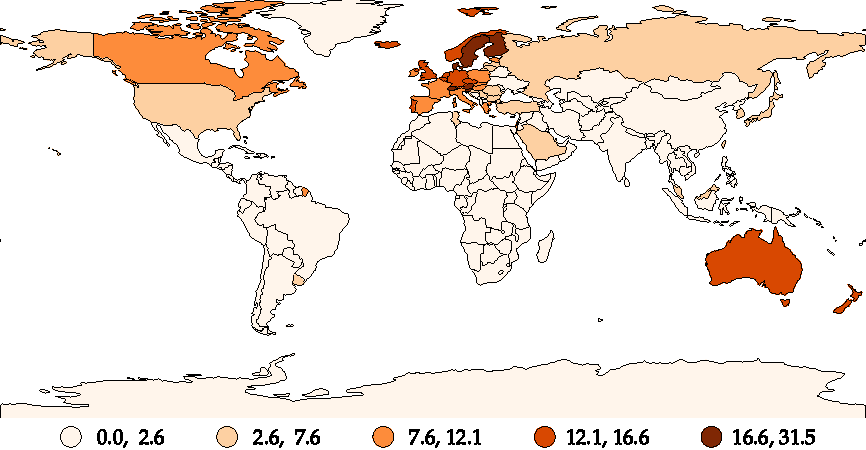
\includegraphics[height=0.8\textheight]{images/nmr-affiliations-per-million-people_naturalbreaks.pdf}

  \(\frac{\text{NMR affiliations}}{\text{million people}}\)
\end{frame}

% Task
\begin{frame}{Our task is to build this machine ourselves!}
  % Schematic of the parts needed to build
\end{frame}

% Main Body
\section{What already works}

\begin{frame}{The power amplifier}

\end{frame}

\begin{frame}{The switch}
\end{frame}


\begin{frame}{Our NMR is affordable \ldots}
  \begin{table}
    \begin{tabular}{@{} lS[table-format=5.2,table-align-text-pre=false] @{}}
      \toprule
      Part                & {Price incl. VAT [CHF]} \\
      \midrule
      Power Amplifier     & 36.01                   \\
      Switch              & 20.05                   \\
      Probe               & {\approx} 15.00         \\
      Low-Noise Amplifier & 73.11                   \\
      Shim Driver         & 257.08                  \\
      Console             & 741.55                  \\
      Magnet              & {\approx} 9000.00       \\
      \bottomrule
      \textbf{Sum}        & \textbf{10142.80}       \\
    \end{tabular}
  \end{table}
  % \freefootnote{2023-09-04}
\end{frame}

\begin{frame}{\ldots{} and competitive}
  \begin{table}
    \begin{tabular}{@{} lrrrl @{}}
      \toprule
                 & Traditional                            & Benchtop                            & \magnethical{}                                                                         &                    \\
      \midrule
      Price      & \numrange[range-phrase=--]{200}{18000} & \numrange[range-phrase=--]{60}{150} & \approx\num{10}                                                                        & k\,CHF             \\
      Frequency  & \numrange[range-phrase=--]{600}{1200}  & \numrange[range-phrase=--]{45}{125} & \num{25}                                                                               & \unit{\mega\hertz} \\
      Resolution & \approx\num{1}                         & \numrange[range-phrase=--]{0.2}{12} & \approx \num{50}\footnote[2]{without shims --- 10x improvement expected with shimming} & \unit{\hertz}      \\
      Weight     & \numrange[range-phrase=--]{600}{15000} & \numrange[range-phrase=--]{5}{1000} & \approx\num{5}                                                                         & \unit{\kilo\gram}  \\
      % \bottomrule
    \end{tabular}
  \end{table}
\end{frame}

% Results
\section{Current measurement capabilities}
\begin{frame}{We can already see a water FID}
  \centering
  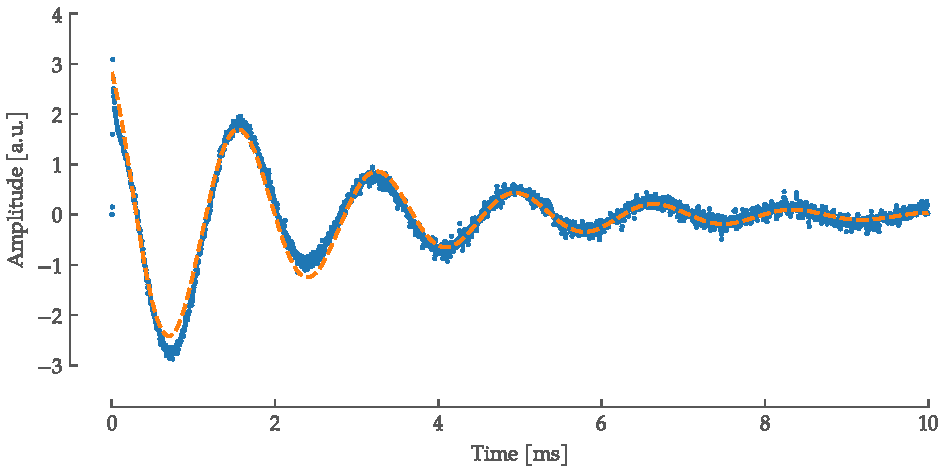
\includegraphics[width=0.9\textwidth]{images/fid_sine_fit.pdf}
\end{frame}

\begin{frame}{\ldots and do a Fourier transform}
  \centering
  \begin{tikzpicture}
    \node (fft)
    {
      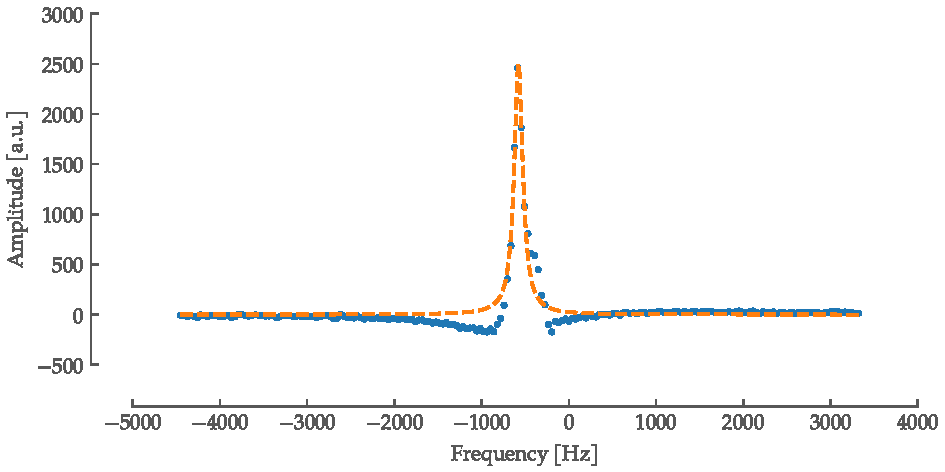
\includegraphics[width=0.9\textwidth]{images/fft_fit.pdf}
    };
    \begin{scope}[overlay]
      \node (structure) at (fft.north)
      [
        anchor=center,
        xshift=0.65cm,
        yshift=0cm
      ]
      {
        \includesvg[height=0.1\textheight]{images/h2o.svg}
      };
      \path[draw=grey,dashed,->] ([yshift=1mm,xshift=-3mm]structure.south east) to ([xshift=0.7cm,yshift=2.5cm]fft.center);
      \path[draw=grey,dashed,->] ([yshift=1mm,xshift=3mm]structure.south west) to ([xshift=0.6cm,yshift=2.5cm]fft.center);
    \end{scope}
  \end{tikzpicture}
\end{frame}

\begin{frame}{Toluene also has a visible signal}
  \centering
  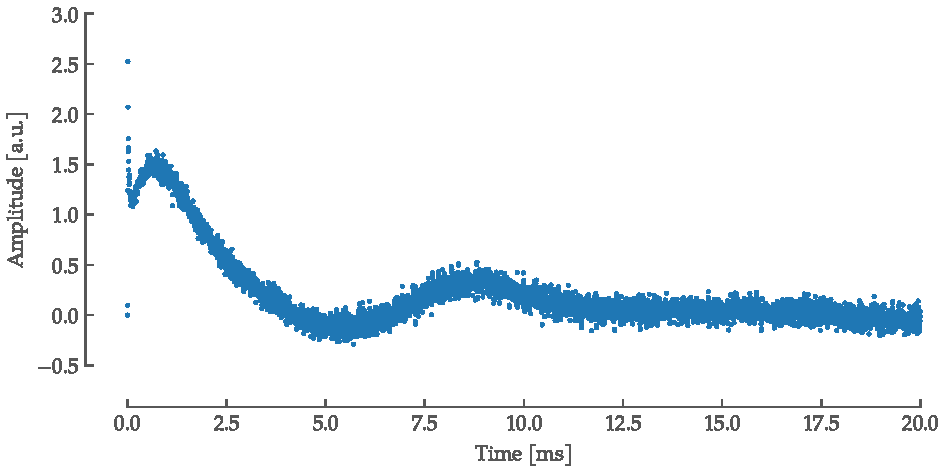
\includegraphics[width=0.9\textwidth]{images/fid_toluene.pdf}
\end{frame}

\begin{frame}{We can even see the Toluene peaks!}
  \centering
  \begin{tikzpicture}
    \node (fft)
    {
      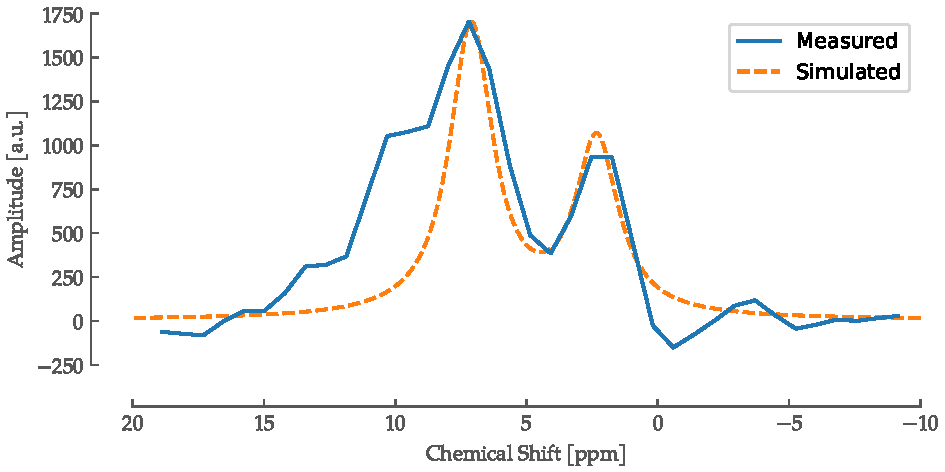
\includegraphics[width=0.9\textwidth]{images/fft_toluene.pdf}
    };
    \begin{scope}[overlay]
      \node (structure) at (fft.north)
      [
        anchor=north west,
        xshift=0mm,
        yshift=1.5cm
      ]
      {
        \includesvg[height=0.15\textheight]{images/toluene.svg}
      };
      \path[draw=grey,dashed,->] ([yshift=5mm,xshift=-4mm]structure.south east) to ([yshift=1.5cm,xshift=1.75cm]fft.center);
      \path[draw=grey,dashed,->] ([yshift=2mm,xshift=2mm]structure.south west) to ([yshift=2.75cm]fft.center);
    \end{scope}
  \end{tikzpicture}
\end{frame}

% Demonstration! Measure FID of water
% TODO: Backup slides with notebook screenshots of measurments
\begin{frame}[standout]
  Demo time!
\end{frame}

% Review
% We've now seen how a measurement works
% I hope I could convince you that the setup is working
% Now the individual parts can be improved individually

\begin{frame}{The setup is working}
  % Now the individual parts can be improved further
\end{frame}

% Conclusion

% Close
\begin{frame}{}
  \begin{center}
    \note[item]{Circling back to the beginning, I would like to end with a quote by E.M. Purcell}
    \emph{
      \enquote{I have not yet lost that sense of wonder, and of delight, that this delicate motion should reside in all ordinary things around us, revealing itself only to him who looks for it.}

      \vspace{2\baselineskip}

      \enquote{There the snow lay around my doorstep -- great heaps of protons quietly precessing in the Earth's magnetic field.}
      % In that on the first snowy, silent night this winter you'll think of the quiet precessions in the earth's magnetic field.
    }
  \end{center}
  \hfill{}--- E.M.\ Purcell
  \note[item]{I wouldn't have thought I would get a glimpse of this wonder that Purcell describes when starting my thesis here, but I'm glad I did.}
  \note[item]{And I hope none of you have lost it yet}
\end{frame}

% End: Show during questions
\begin{frame}{Thank you!}
  \begin{columns}
    \begin{column}{0.5\textwidth}
      \centering
      \includesvg[width=0.5\textwidth]{./images/logo_magnETHical.svg}
    \end{column}
    \begin{column}{0.5\textwidth}
      \centering
      Find everything on \\ \vspace*{\baselineskip}

      \includesvg[width=0.5\textwidth]{./images/gitlab_qrcode.svg}

      \url{https://gitlab.ethz.ch/mstabel/nmr-spectrometer}
    \end{column}
  \end{columns}
\end{frame}


%%%%%%%%%%%%%%%%%%%%%%%%%%%%%%%%%%%%%%%%%%%%%%%%%%%%%%%%%%%%%%%%%%%%%%%%%%%%%%%
% Appendix / Backup Slides
%%%%%%%%%%%%%%%%%%%%%%%%%%%%%%%%%%%%%%%%%%%%%%%%%%%%%%%%%%%%%%%%%%%%%%%%%%%%%%%

\appendix

\begin{frame}[standout]
  Backup
\end{frame}


\begin{frame}{Simple Pulse Sequence}
  \centering
  \includesvg[width=0.5\textwidth]{simple_pulse_sequence.svg}
\end{frame}

\begin{frame}{Rabi nutation of water}
  \centering
  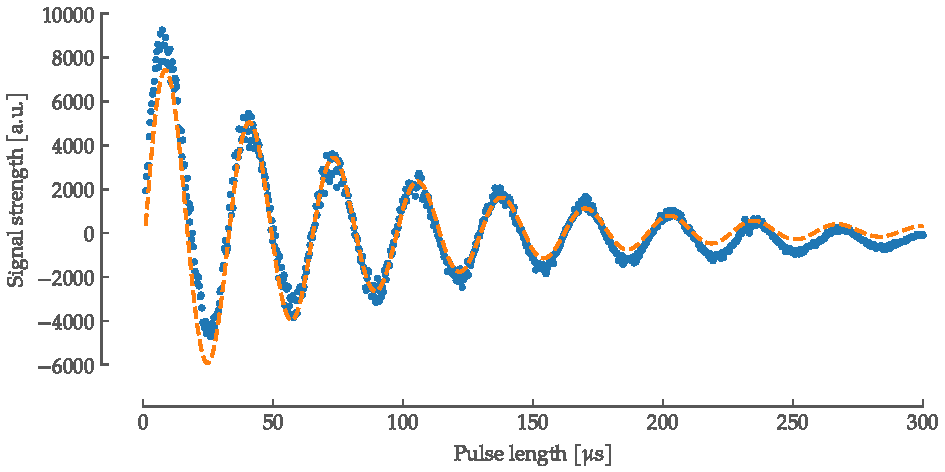
\includegraphics[width=0.9\textwidth]{rabi_nutation_fit.pdf}
  \note[item]{\(T_{period} = \qty{32}{\micro\second}\)}
  \note[item]{\(T_{\frac{\pi}{2}} = \qty{8}{\micro\second}\)}
\end{frame}

\begin{frame}{Spin Echo Animation}
  \centering
  \movie[width=9cm,height=6.75cm,poster]{}{./hahn_echo_cc_gwm.gif}
  \freefootnote{\href{https://commons.wikimedia.org/wiki/File:GWM_HahnEcho.gif}{Gavin Morley - CC BY-SA 3.0}}
\end{frame}

\begin{frame}{T2 Decay Animation}
  \centering
  \movie[width=9cm,height=6.75cm,poster]{}{./hahn_echo_decay_cc_gwm.gif}
  \freefootnote{\href{https://commons.wikimedia.org/wiki/File:GWM_HahnEchoDecay.gif}{Gavin Morley - CC BY-SA 3.0}}
\end{frame}

\begin{frame}{Spin Echo Sequence}
  \centering
  \includesvg[width=0.9\textwidth]{spin_echo_sequence.svg}
\end{frame}

\begin{frame}{T2 decay of water}
  \centering
  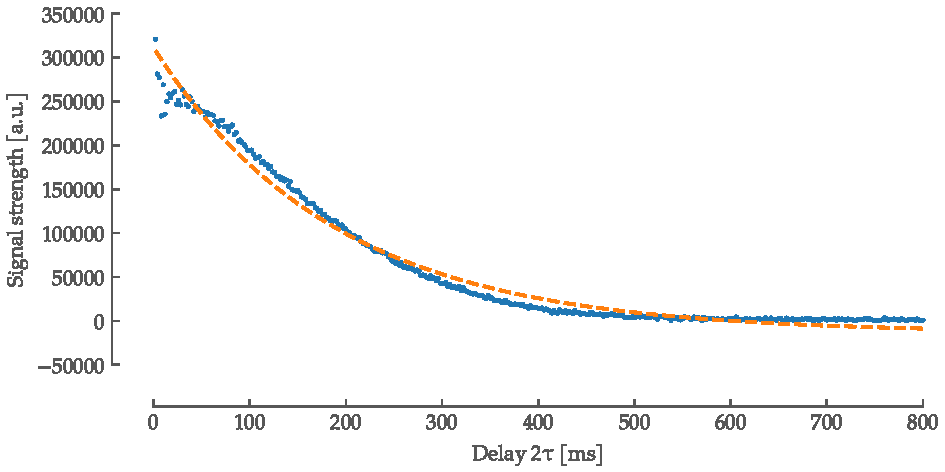
\includegraphics[width=0.9\textwidth]{t2_decay_fit.pdf}
  \note[item]{\(T_2 = \qty{190}{\milli\second}\)}
\end{frame}

\end{document}